\documentclass{beamer}
%\documentclass[handout]{beamer}
\usepackage{hyperref}
\usepackage[labelformat=empty]{caption}
\usepackage{color}
\usepackage{tipa}
\usepackage{gb4e}

\usepackage{media9}

\definecolor{greenish}{HTML}{00A08A}
\definecolor{pinkish}{HTML}{FF0000}
\definecolor{yellowish}{HTML}{F2AD00}
\definecolor{orangish}{HTML}{F98400}
\definecolor{bluish}{HTML}{5BBCD6}

\usetheme{default}
\usefonttheme{professionalfonts}
\usecolortheme{seagull}
%\useoutertheme[subsection=false,section=false]{miniframes}
\setbeamercolor{frametitle}{fg=white, bg=pinkish}
\setbeamercolor{title}{fg=white, bg=pinkish}
\setbeamercovered{transparent}
\resetcountonoverlays{excnt}
\setbeamercolor{alerted text}{fg=pinkish}


\title[ELAN]{Introduction to ELAN}
\author[Bradley McDonnell]{Bradley McDonnell}
%\institute[UCSB]{CoLang 2012, University of Kansas}
\date{March 10, 2020}
  
\begin{document}
  \section{Course Overview}
    \begin{frame}
    \titlepage
    \end{frame}
    
    \begin{frame}{Goals}
      \begin{enumerate}
        \item<1-> Navigate ELAN files
        \item<2-> Produce/edit annotations in ELAN
        \item<3-> Create/edit tiers in ELAN
        \item<4-> Conceptualize \& annotate your own recordings
      \end{enumerate}
    \end{frame}
        
%    \begin{frame}{syllabus: day one}
%      \begin{enumerate}
%         \item<1-> A tour of ELAN
%         \item<2-> Nuts \& bolts: downloading/installation, file storage
%         \item<3-> Conceptualizing transcripts
%         \item<4-> Creating a single-language annotation file with one speaker
%       \begin{itemize}
%         \item<4-> Exercise 1: One speaker in one language
%       \end{itemize}
%      \item<5-> Creating a single-language annotation file with multiple speakers
%        \begin{itemize}
%          \item<5-> Exercise 2: Multiple speakers in one language
%        \end{itemize}
%      \end{enumerate}
%    \end{frame}
%    
%    \begin{frame}{syllabus: day two}
%      \begin{enumerate}
%        \item Review Day 1
%        \item Parent \& child tiers, linguistic (stereo)types, \& tier behaviors
%        \item Creating a two language simple annotation file  (sentence level) with one speaker
%        \begin{itemize}
%          \item Exercise 3: One speaker in two languages
%        \end{itemize}
%      \end{enumerate}
%    \end{frame}
%    
%    \begin{frame}{syllabus: day three}
%      \begin{enumerate}
%        \item Review Days 1 \& 2
%        \item More on parent \& child tiers, linguistic (stereo)types, \& tier behaviors
%        \item Creating a two language complex annotation (interlinearized gloss) 
%       \begin{itemize}
%          \item Exercise 4: One speaker in two languages with IGT
%        \end{itemize}
%      \end{enumerate}
%    \end{frame}    
%    
%    \begin{frame}{syllabus: day four}
%      \begin{enumerate}
%            \item Working with a single video file
%        \begin{itemize}
%          \item Exercise 5: Working with a single video camera
%        \end{itemize}
%      \item Working with multiple video \& audio files
%        \begin{itemize}
%          \item Exercise 6: Working with multiple video cameras \& a separate audio file
%        \end{itemize}
%      \item Some advanced features of ELAN: Template, Gaps, Silence%
%        \begin{itemize}
%          \item Exercise 7: Some tricks for automating transcription
%        \end{itemize}
%      \end{enumerate}
%    \end{frame}
%    
%    \begin{frame}{what to expect for ELAN 2}
%      Level 2 will be focused on more advanced features of ELAN. These include:
%      \pause
%      \begin{enumerate}
%      \item<2-> specialized \texttt{`modes'} for segmentation \& transcription,
%      \item<3-> searching \& manipulating data,
%      \item<4-> importing/exporting ELAN files from/to other working \& presentation formats
%      \end{enumerate}
%    \end{frame}
    
    \section{nuts \& bolts}
    % \begin{frame}{downloading ELAN}
    %    \begin{figure}[htbp]
    %    \begin{center}
    %      \caption*{\url{https://tla.mpi.nl/tools/tla-tools/elan/download/}}
    %      \setlength\fboxsep{0pt}
    %      \setlength\fboxrule{0pt}
    %      \fbox{\includegraphics[scale=0.2]{img/ELAN-Download.png}}
    %   \end{center}
    %   \end{figure}
    % \end{frame}
    
    % \begin{frame}{downloading \& installing}
    %   \begin{enumerate}
    %     \item For Windows: 
    %       \begin{itemize}
    %         \item Double click on {\color{blue}\underline{\textbf{ELAN 5.1 Windows}}},
    %         \item Follow the installer instructions.\\
    %         \item []
    %       \end{itemize}
    %     \item For Mac:
    %       \begin{itemize}
    %         \item Double click on {\color{blue}\underline{\textbf{ELAN 5.1 MacOS X}}},
    %         \item Follow the installer instructions.
    %         \item You may need to drag the \texttt{ELAN 5.1} folder into \texttt{Applications} folder
    %       \end{itemize}
    %   \end{enumerate}
    % \end{frame}    
    
%    \begin{frame}{file storage during the course}
%      \begin{enumerate}
%      \item[] Please save everything you complete in class on your thumb drive and/or laptop. You will be using them later in the course and beyond.
%      \end{enumerate}
%    \end{frame}
    
    \section{Introduction to ELAN}
    \begin{frame}{what is a time-aligned transcript?}
      \begin{enumerate}
      \item<2-> Time-aligned transcriptions match:
        \begin{itemize}
        \item<3-> sections of text (ANNOTATIONS) to
        \item<4-> pieces of audio and/or video recordings (MEDIA).
        \end{itemize} 
      \end{enumerate}
     \uncover<5->{
      \begin{figure}[h!]
        \begin{center}
          \setlength\fboxsep{0pt}
          \setlength\fboxrule{0pt}
            \href{run:audio/waveform-audio.wav}{\fbox{\includegraphics[scale=0.4]{img/waveform1.png}}}
       \end{center}
       \end{figure}
      % \includemedia[
      % label=waveform-audio,
      % width=1\textwidth,
      % addresource=audio/waveform-audio.wav, 
      % transparent, 
      % activate=onclick,
      % flashvars={
      % source=audio/waveform-audio.wav
      % &loop=false % loop video
      % &scaleMode=letterbox 
      % }
      % ]{\includegraphics[scale=0.4]{img/waveform1.png}}{VPlayer.swf}
      
     \begin{center}
      \begin{tabular}{|ll|}
      \hline
        \textbf{Jack:} &  Hola.\\
        \textbf{Kristen:} & Hey!\\
        \textbf{Jake:} & What up.\\
        \textbf{Jack:} & How's it going?\\
        \textbf{Jake:} & Good.\\
      \hline
      \end{tabular}
      \end{center}
      }
    \end{frame}

    \begin{frame}{what is a time-aligned transcript?}
      \begin{enumerate}
      \item Time-aligned transcriptions match:
        \begin{itemize}
        \item sections of text (ANNOTATIONS) to
        \item pieces of audio and/or video recordings (MEDIA).
        \end{itemize} 
      \end{enumerate}
      \begin{figure}[htbp]
       \begin{center}
         \setlength\fboxsep{0pt}
         \setlength\fboxrule{0pt}
         \href{run:audio/waveform-audio.wav}{\fbox{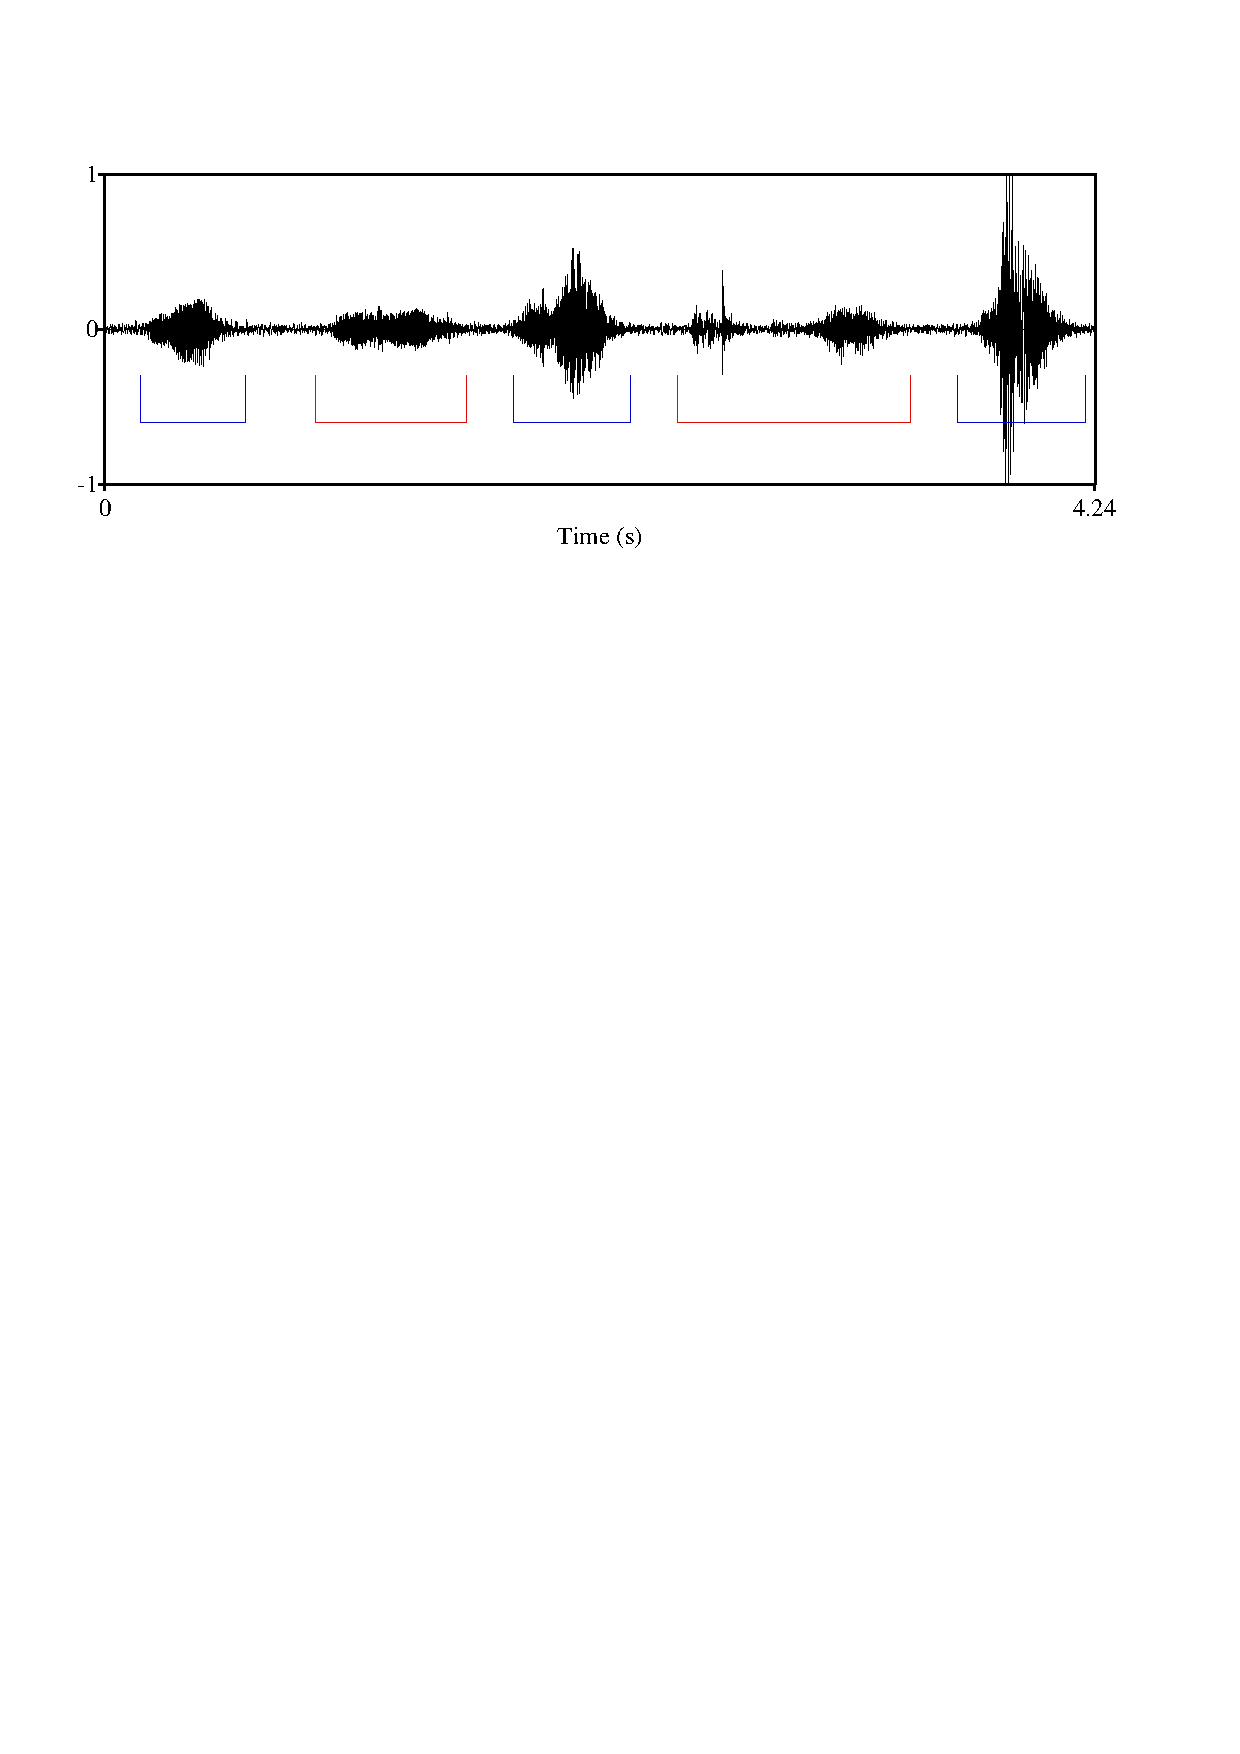
\includegraphics[scale=0.4]{img/waveform2.png}}}
      \end{center}
      \end{figure}
     \begin{center}
      \begin{tabular}{|ll|}
      \hline
        \textbf{Jack:} &  Hola.\\
        \textbf{Kristen:} & Hey!\\
        \textbf{Jake:} & What up.\\
        \textbf{Jack:} & How's it going?\\
        \textbf{Jake:} & Good.\\
      \hline
      \end{tabular}
      \end{center}
    \end{frame}     
      
    \begin{frame}{time-aligned transcripts}
      \begin{enumerate}
      \item<1-> What are some common time-aligned transcriptions? 
        \begin{itemize}
          \item<2-> closed captioning
          \item<3-> subtitles
          \item<4-> \ldots
        \end{itemize} 
      \end{enumerate}
    \end{frame}
    
    \begin{frame}{why bother?}
    \uncover<2->{Your language resources will be much richer. Your resources:}
      \begin{enumerate}
        \item<3-> are searchable
        \item<4-> are verifiable
        \item<5-> reinforce your language as a living language
        \item<6-> match orthography to pronunciation for literacy
        \item<7-> \ldots
      \end{enumerate}
    \end{frame}
    
    \begin{frame}{what is ELAN?}
      \uncover<2->{ELAN is a tool for producing time-aligned transcripts of audiovisual recordings.}
      \begin{enumerate}
        \item<3-> Developed \& maintained by the Max Planck Institute for Psycholinguistics in Nijmegen. 
        \item<4-> ELAN stands for \textbf{E}UDICO \textbf{L}inguistic \textbf{An}notator.
        \item<4-> EUDICO stands for the \textbf{Eu}ropean \textbf{Di}stributed \textbf{Co}rpus Project.
        \item<5-> It is developed alongside a number of other software tools that work in concert with ELAN (i.e., Arbil for metadata \& Lexus for lexical databases).  
      \end{enumerate}
    \end{frame}

    \begin{frame}{why use ELAN?}
      \begin{enumerate}
        \item<2-> ELAN uses non-proprietary, standards-compliant output.
          \begin{itemize}
            \item<3-> It uses {\color{blue}\textbf{unicode}} so that your fonts display correctly.
            \item<4-> It uses {\color{blue}\textbf{XML}} so that your document is long-lasting and archive ready. It conforms to well documented XML schema and is human eyeball-readable.  
          \end{itemize}
        \item<5-> ELAN documents can be exported to a wide range of useful products for a wide range of audiences.        
          \begin{itemize}
            \item<6-> ELAN can be exported as a subtitled video for communities.
            \item<7-> ELAN can also be exported to Praat, FLEx, Toolbox, Subtitled text, etc\ldots for linguists.
          \end{itemize}
      \end{enumerate}
    \end{frame}
    
    \begin{frame}{how is ELAN better than a printed transcript?}
      \begin{enumerate}
      \item<2-> There are many uses for printed transcripts.
      \item<3-> In the past, the printed transcript was considered the primary source:
        \begin{itemize}
          \item<4-> Whatever the printed transcript could not capture was not included in the discussion.
          \item<4-> An accompanying recording was just considered to be an added bonus.
        \end{itemize}
      \item<5-> In ELAN the text \& the recording are \texttt{unified}.
        \begin{itemize}
          \item<6-> This opens up a number of possibilities for research \& learning.
        \end{itemize}
      \item<7-> The printed transcript is one of the many possible exports in ELAN.
      \end{enumerate}
    \end{frame}
    
    \begin{frame}{what does ELAN \textsc{not} do?}
      \begin{enumerate}
        \item<1-> ELAN is \textsc{not} a media editor: it cannot change your audio/video files.
          \begin{itemize}
            \item<2-> This is actually a good thing \ldots we won't inadvertently change our precious recordings.
            \item<2-> There are many other programs that can do this (i.e., Audacity).
          \end{itemize}
        \item<3-> ELAN is \textsc{not} a text editor: its annotations and outputs are in \texttt{plain text}.
          \begin{itemize}
            \item<4-> In order to format text with \underline{underlining}, \textit{italics}, \textsc{small caps}, or \textbf{bolding}, you will need to use a text editor after you export your annotations.   
          \end{itemize}
      \end{enumerate}
    \end{frame}
        
  \section{ELAN basics}
    \begin{frame}{the panes of ELAN}
       \begin{figure}[htbp]
       \begin{center}
         \setlength\fboxsep{0pt}
         \setlength\fboxrule{0pt}
         \fbox{\includegraphics[scale=0.5]{img/ElanWindow.png}}
      \end{center}
      \end{figure}
    \end{frame}
    
    \begin{frame}{some foundational concepts}
      \begin{enumerate}
        \item<1-> To use ELAN effectively, you must understand:
          \begin{itemize}
            \item<2-> Your own goals for the structure of your transcript.
            \item<3-> ELAN's built in concepts about different kinds of annotations.
            \item<4-> How your goals maps onto ELAN's concepts.
          \end{itemize}
      \end{enumerate}
      \begin{figure}[t]
      \setlength{\unitlength}{1cm}
      \begin{center}
      \begin{picture}(12, 1)
          % Symbolic association upper left corner
          \uncover<2->{\put(1,1){Your Goals}}
          \uncover<3->{\put(7,1){ELAN's Concepts}}
          \uncover<5->{\put(3.05,0){Successful ELAN Project}}
          \thicklines
          \uncover<4->{\put(2.5,0.9){\vector(1,-1){0.5}}
          \put(7.6, 0.9){\vector(-1,-1){0.5}}}
       \end{picture}
       \end{center}
       \end{figure}
      \begin{enumerate}
      \setcounter{enumi}{1}
        \item<6-> With this in mind, let's ask ourselves:
          \begin{itemize}
            \item<7-> \textit{What kind of information do I want in my time-aligned transcript?}
          \end{itemize}
        \item<8-> Let's consider what we see in some printed transcripts.
      \end{enumerate} 
    \end{frame}
    
    \begin{frame}{the structure of your transcript}
      \begin{description}
        \item<1->[Example 1:] Single language with one speaker\\(simple transcription system).
        \item<1->[]
        \item<2->[] ((JAY-Z Fresh Air Interview))\footnote{\tiny\url{http://www.npr.org/2010/11/16/131334322/the-fresh-air-interview-jay-z-decoded}}
        \item<2->[\href{run:audio/Jay-Z.wav}{JAY-Z:}] ``Well I had a - I grew up in the Marcy Projects in Brooklyn, and my mom and pop had an extensive record collection. So Michael Jackson and Stevie Wonder, and all those sounds and souls - and Motown etc., etc. - filled the house. So I was very familiar with the song when Kanye bought me the sample. It was just such an interesting and fresh take on it that I immediately was drawn to it.''
      \end{description}
    \end{frame}
    
    \begin{frame}{the structure of your transcript}
      \begin{description}
      \item<1->[Example 2:] Single language with multiple speakers\\(more informative transcription system).
        \begin{enumerate}
          \item<2-> Prosodic phrasing
          \item<2-> Speaker overlap
          \item<2-> Pause length
          \item<2-> Laughter \& other non-language oral noises
          \item<2-> Phrase accent/stress
        \end{enumerate}
      \item<3->[Note:] The following example is in the UCSB transcription system.
      \end{description}
    \end{frame}
    
     \begin{frame}{the structure of your transcript}
     \href{run:audio/TwoSpeaker.m4a}{\hspace{6pt}{\color{black}\tiny ((\textit{Fish Tacos}, English))}}
       \begin{figure}[h!]
       \begin{flushleft}
         \setlength\fboxsep{0pt}
         \setlength\fboxrule{0pt}
         {\fbox{\includegraphics[scale=0.4]{img/TwoSpeaker.png}}}
      \end{flushleft}
      \end{figure}
    \end{frame}
    
     \begin{frame}{the structure of your transcript}
     \begin{description}
       \item<1->[Example 3:] Two languages
         \begin{enumerate}
           \item<2-> Subject language
           \item<2-> Translation language
           \item<2-> Sentence level translation
         \end{enumerate}
     \end{description}
     \uncover<3->{\href{run:audio/TwoLanguage.wav}{\scriptsize ((\textit{Polygamous Marriage}, Shona))}
       \begin{figure}[t]
       \begin{flushleft}
         \setlength\fboxsep{0pt}
         \setlength\fboxrule{0pt}
         {\fbox{\includegraphics[scale=0.7]{img/TwoLanguage.png}}}
      \end{flushleft}
      \end{figure}}
    \end{frame}
    
    \begin{frame}{the structure of your transcript}
      \begin{description}
      \item<1->[Example 4:] Two languages with full IGT:
        \begin{enumerate}
          \item<2-> Subject language
          \item<2-> Translation language
          \item<2-> Prosodic phrases
          \item<2-> Morphemes
          \item<2-> Morpheme glosses
          \item<2-> Sentence level translations
        \end{enumerate}
      \end{description}
    \end{frame}
    
    \begin{frame}{the structure of your transcript}
  \href{run:audio/FullIGT.wav}{\scriptsize ((\textit{Guava}, Besemah))}
       \begin{figure}[h!]
       \begin{flushleft}
         \setlength\fboxsep{0pt}
         \setlength\fboxrule{0pt}
         {\fbox{\includegraphics[scale=0.7]{img/FullIGT.png}}}
      \end{flushleft}
      \end{figure}
    \end{frame}
    
   \begin{frame}{tiers \& types}
      \begin{enumerate}
        \item<1-> A \texttt{tier} is everything from a transcript that is the same kind of information.
          \begin{itemize}
            \item<2-> everything that Jay-Z said in example 1.
            \item<2-> everything that Jack said in example 2. 
            \item<2-> everything labeled Intonation Unit (or Gloss, etc.) in example 3.
          \end{itemize}
        \item<3-> With printed transcripts we are forced to put different parts of a single tier on different lines.
      \end{enumerate}
      \uncover<4->{
      \begin{center}
      \begin{tabular}{|llllll|}
      \hline
      \multicolumn{2}{|l}{\ } &  \multicolumn{2}{l}{}&  \multicolumn{2}{l|}{}\\
      Tier 1: & \dots &  &  & Tier 1: & \ldots\\
      Tier 2: & \dots & &  & Tier 2: & \ldots\\
      Tier 3: & \dots & &  & Tier 3: & \ldots\\
      &&&&&\\
      Tier 1: & \dots & &  & Tier 1: & \ldots\\
      Tier 2: & \dots &  &  & Tier 2: & \ldots\\
      Tier 3: & \dots &  &  & Tier 3: & \ldots\\
      &&&&&\\      
      \hline
      \end{tabular}
      \end{center}}
    \end{frame}
    
    \begin{frame}{tiers \& types}
      \begin{enumerate}
        \item[]<1-> With a time-based tool like ELAN, we can conceive of each tier as existing 
          \begin{itemize}
            \item<2-> as a \textbf{continuous} stream on a single line, 
            \item<2-> \textbf{contiguous} to the timeline of the media.
          \end{itemize}
      \end{enumerate}
      \uncover<3->{
       \begin{figure}[htbp]
       \begin{center}
         \setlength\fboxsep{0pt}
         \setlength\fboxrule{0pt}
         \fbox{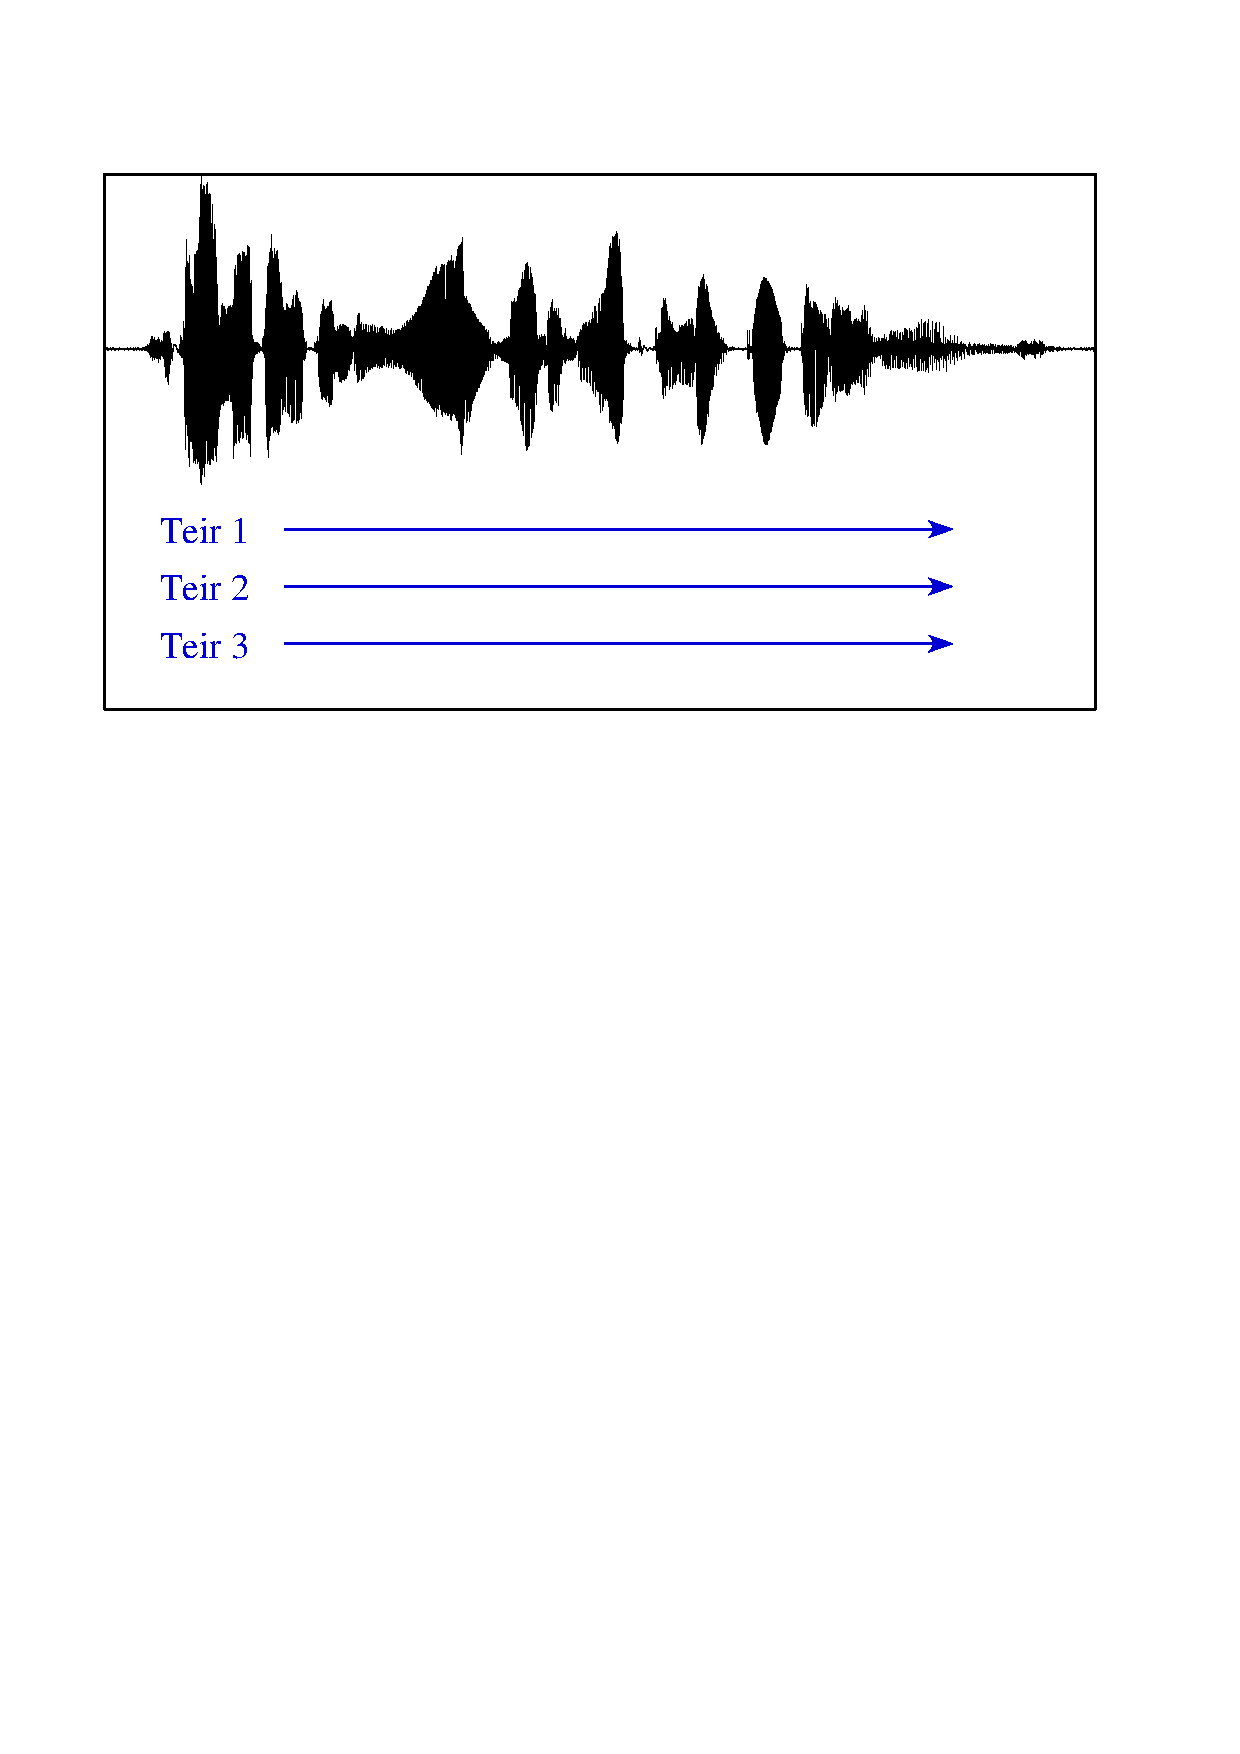
\includegraphics[scale=0.5]{img/tiers1.png}}
      \end{center}
      \end{figure}}
    \end{frame}
    
    \begin{frame}{tiers \& types}
With multiple continuous tiers, we can capture overlap between speakers.
       \uncover<2->{
       \begin{figure}[htbp]
       \begin{center}
         \setlength\fboxsep{0pt}
         \setlength\fboxrule{0pt}
         \fbox{\includegraphics[scale=0.5]{img/overlap.png}}
      \end{center}
      \end{figure}}
    \end{frame}
    
     \begin{frame}{tiers \& types}
       \begin{enumerate}
         \item<1-> By conceiving of tiers as progressing forward through time, we can begin to establish some relationships between different tiers. 
         \item<2-> The parent-child relationship between tiers:
           \begin{description}
             \item<3->[Parents:] tiers that control the behavior of other (child) tiers in some way.
             \item<3->[Children:] tiers that are associated with and dependent upon other (parent) tiers.
           \end{description}
         \item<4-> This parent-child relationship is recursive, so a child of one tier could be the parent of another tier.
         \item<5-> Certain changes to parent tiers will affect child tiers. 
       \end{enumerate}
    \end{frame}
    
    \begin{frame}{tiers \& types}
    \begin{enumerate}
      \item<1-> Top-level parent tiers are directly associated to the recording.
        \begin{itemize}
          \item<2-> This top-level tier is usually a direct representation of the media.
          \item<2-> Every ELAN file has at least one of these tiers.
        \end{itemize}
    \end{enumerate}
      \uncover<3->{
      \begin{figure}[htbp]
       \begin{center}
         \setlength\fboxsep{0pt}
         \setlength\fboxrule{0pt}
         \fbox{\includegraphics[scale=0.5]{img/tiers.png}}
      \end{center}
      \end{figure}}
    \end{frame}
    
   \begin{frame}{tiers \& types}
    \begin{enumerate}
      \item<1-> The precise relationship between a parent \& a child tier is defined in ELAN by \texttt{linguistic types}.
      \item<2-> The linguistic type is determined by the kind of data a tier contains:
        \begin{itemize}
          \item<3-> Utterances 
          \item<3-> Translations
          \item<3-> Linguistic analysis
          \item<3-> \ldots
        \end{itemize}
      \item<4-> The linguistic type usually determines a one-to-one or one-to-many relationship between the parent \& child tier.
      \item<5-> There are some restrictions on what linguistic types can be parent tiers.
    \end{enumerate}
   \end{frame}
    
   \begin{frame}{let's get started\ldots}
      \begin{figure}[htbp]
      \begin{center}
         \setlength\fboxsep{0pt}
         \setlength\fboxrule{0pt}
         \fbox{\includegraphics[scale=1\textwidth]{img/cry.png}}
      \end{center}
      \end{figure}
   \end{frame}
   
     \section{Types}
    \begin{frame}{types (stereotypes) vs. tiers}
    \begin{itemize}
      \item Every tier is assigned to a linguistic type
      \item The linguistic type specifies the stereotypical constraints of that tier
    \end{itemize}
    \pause
      \begin{figure}[h!]
      \begin{center}
      \caption{the default stereotype}
         \setlength\fboxsep{0pt}
         \setlength\fboxrule{0pt}
         \fbox{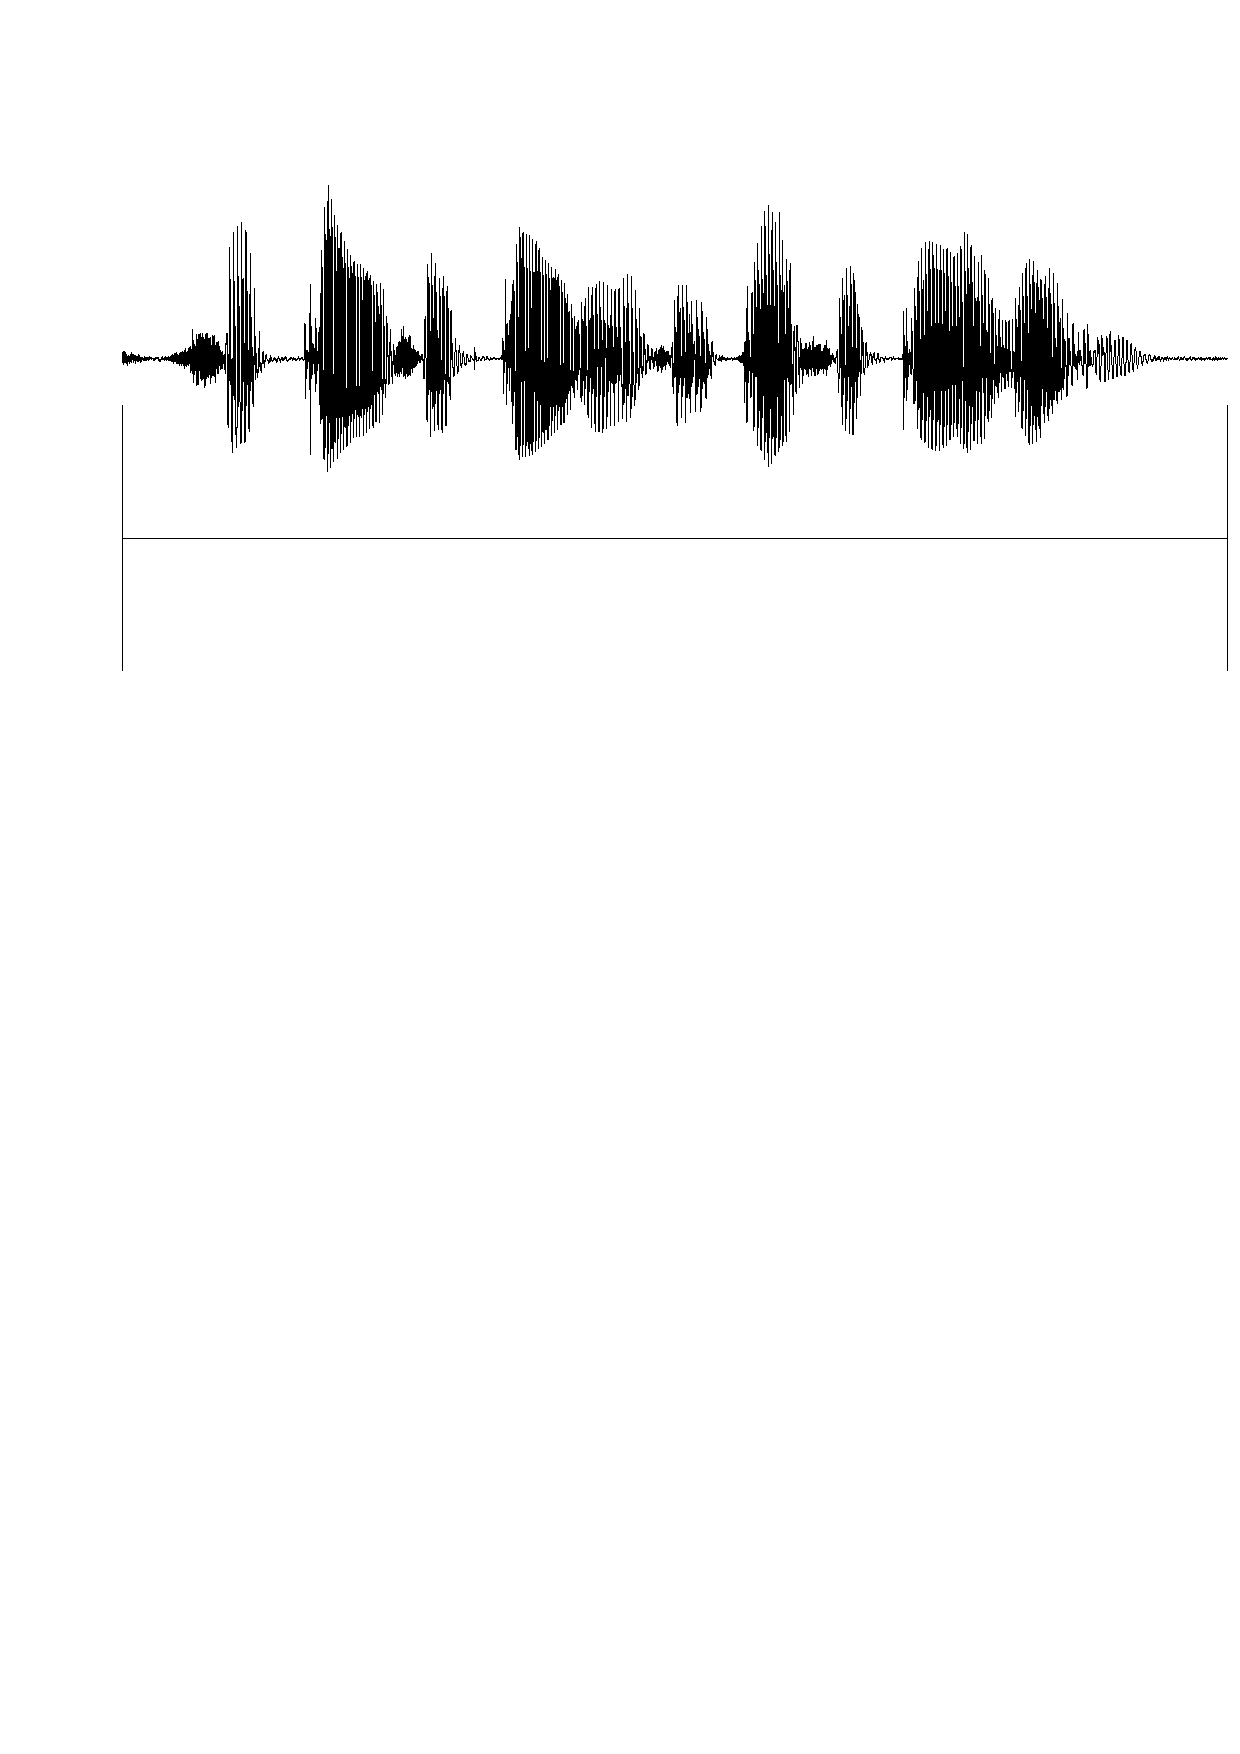
\includegraphics[scale=0.5]{img/default.png}}
      \end{center}
      \end{figure}
    \end{frame}
    
    \begin{frame}{types (stereotypes) vs. tiers}
      \pause
      \begin{figure}[t]
      \setlength{\unitlength}{1cm}
      \begin{center}
      \begin{picture}(12, 8)
          % Symbolic association upper left corner
          \put(1,5.5){Symbolic Association}
          \put(0,7){\line(0,1){0.9}}
          \put(5,7){\line(0,1){0.9}}
          \put(0,7.5){\line(1,0){5}}
          \put(0,6){\line(0,1){0.9}}
          \put(5,6){\line(0,1){0.9}}
          \put(0,6.5){\line(1,0){5}}
        \pause    
          % Symbolic subdivision lower right corner
          \put(7,1.5){Symbolic Subdivision}
          \put(6,2){\line(0,1){0.9}}
          \put(11,2){\line(0,1){0.9}}
          \put(9.5,2){\line(0,1){0.9}}
          \put(7.5,2){\line(0,1){0.9}}
          \put(6,2.5){\line(1,0){5}}
          \put(6,3){\line(0,1){0.9}}
          \put(11,3){\line(0,1){0.9}}
          \put(6,3.5){\line(1,0){5}}
        \pause
          % Included-in lower left corner
          \put(2,1.5){Included In}
          \put(0,3){\line(0,1){0.9}}
          \put(5,3){\line(0,1){0.9}}
          \put(5,3){\line(0,1){0.9}}
          \put(0,3.5){\line(1,0){5}}
          \put(1,2){\line(0,1){0.9}}
          \put(3,2){\line(0,1){0.9}}
          \put(5,2){\line(0,1){0.9}}
          \put(4,2){\line(0,1){0.9}}
          \put(1,2.5){\line(1,0){2}}
          \put(4,2.5){\line(1,0){1}}
       \pause    
          % Time subdivision upper right corner
          \put(7,5.5){Time Subdivision}
          \put(6,6){\line(0,1){0.9}}
          \put(11,6){\line(0,1){0.9}}
          \put(8.5,6){\line(0,1){0.9}}
          \put(10,6){\line(0,1){0.9}}
          \put(7,6){\line(0,1){0.9}}
          \put(6,6.5){\line(1,0){5}}
          \put(6,7){\line(0,1){0.9}}
          \put(11,7){\line(0,1){0.9}}
          \put(6,7.5){\line(1,0){5}}
       \end{picture}
       \end{center}
       \end{figure}
    \end{frame}
   
   \begin{frame}{exercise \#1}
    \begin{itemize}
      \item<1-> In this exercise we will learn:
        \begin{enumerate}
          \item<2-> How to create a new ELAN file from a recording
          \item<3-> How to enter time-aligned text on the default tier
          \item<4->How to edit time-aligned text
          \item<5-> How to save an ELAN file
        \end{enumerate}
%      \item<6-> Go to: \url{http://uweb.ucsb.edu/\~bjm/ELAN1/}
%      \item<7-> Download \texttt{Ex1.zip} \& extract the files
    \end{itemize}
   \end{frame} 
   
   \begin{frame}{exercise \#2}
    \begin{itemize}
      \item<1-> In this exercise we will learn:
        \begin{enumerate}
          \item<2-> How to create additional tiers
          \item<3-> How to work with overlapping speech
          \item<4-> A little about linguistic types
        \end{enumerate}
%      \item<5-> Go to: \url{http://uweb.ucsb.edu/\~bjm/ELAN1/}
%      \item<6-> Download \texttt{Ex2.zip} \& extract the files
    \end{itemize}
   \end{frame} 
   
   \begin{frame}{exercise \#3}
    \begin{itemize}
      \item<1-> In this exercise we will learn:
        \begin{enumerate}
          \item<2-> How to conceive of and create additional linguistic types \& tiers
          \item<3-> How to work with two languages:
            \begin{itemize}
              \item<4-> A subject language
              \item<4-> A translation language
            \end{itemize}
        \end{enumerate}
%      \item<5-> Go to: \url{http://uweb.ucsb.edu/\~bjm/ELAN1/}
%      \item<6-> Download \texttt{Ex3.zip} \& extract the files
    \end{itemize}
   \end{frame} 

%    \begin{frame}{exercise \#4}
%     \begin{itemize}
%       \item<1-> In this exercise we will learn:
%         \begin{enumerate}
%           \item<2-> How to create additional linguistic types for IGT          
%           \item<3-> How to work with numerous tiers
%         \end{enumerate}
%       \item<4-> Go to: \url{http://uweb.ucsb.edu/\~bjm/ELAN1/}
%       \item<5-> Download \texttt{Ex4.zip} \& extract the files
%     \end{itemize}
%    \end{frame} 
%    
%           
%           
%           
%    %%%%%%%%%%%%%%%%%%%%%%%%%%%%%%%%%%%%%%%%%% 
%     \begin{frame}{overview}
%       \begin{enumerate}
%         \item<1-> The final product - an example of a fully annotated ELAN file
%         \item<2-> Navigating ELAN - the panes/controls of ELAN 
%         \item<3-> Annotations - creating, editing, deleting annotations
%         \item<4-> Tiers - creating, editing, copying, deleting tiers
%         \item<5-> Types - creating, editing, deleting types
%         \item<6-> Starting from scratch with audio/video
%         \item<7-> Starting with a templates - saving, opening templates
%         \item<8-> Begin your own projects \ldots
%       \end{enumerate}
%     \end{frame}
%     
% 
%     
%     \begin{frame}{exercise \#1 - basics}
%       NAVIGATE EX \#1 BIKE-SHOP \& EX \#1 DURIAN\\
%       \begin{enumerate}
%         \item play inside/outside of annotation (with loop mode)
%         \item select/move between annotations 
%         \item select/move between tiers
%         \item zoom in/out
%         \item turn down the volume
%         \item slow the playback rate
%         \item check out the shortcut keys: \url{http://www.lat-mpi.eu/tools/elan/manual/ch09s02s02.html}
%       \end{enumerate}
%     \end{frame}
%     
%   \section{Annotations}
%     \begin{frame}{editing annotations}
%       \begin{enumerate}
%         \item<1-> create, delete, move, edit (content \& length) annotations
%         \item<2-> copy annotations
%         \item<3-> enter annotation inline \& in annotation box
%         \item<4-> delete annotation value
%         \item<5-> split/merge annotations
%       \end{enumerate}
%     \end{frame}
%     
%     \begin{frame}{exercise \#2 - editing annotations}
%       PRACTICE WITH EX \#2 FISH TACOS 
%       \begin{enumerate}
%         \item create \textit{6} annotations that are missing in the first 30 seconds
%         \item type the missing text into the annotation box  
%         \item combine any two annotations
%         \item split any one annotation
% 	 \end{enumerate}
% 	 \pause
% 	 PRACTICE WITH EX \#2 DURIAN
% 	 \begin{enumerate}
%         \item move \textit{3} annotations that are in the wrong place
%         \item shorten \textit{2} annotations that are too long
%         \item lengthen \textit{2} annotations that are too short
%       \end{enumerate}
%     \end{frame}
%     
%   \section{Tiers}
%     \begin{frame}{editing tiers part one}
%       \begin{enumerate}
%         \item<1-> rename an existing tier
%         \item<2-> copy an existing tier
%         \item<3-> delete original tier
%         \item<4-> add a new participant
%         \item<5-> change the parent of a tier
%       \end{enumerate}
%     \end{frame}
%     
%     \begin{frame}{exercise \#3 - editing tiers}
%     PRACTICE WITH EX \#3 BIKE SHOP
%       \begin{enumerate}
%         \item delete the \textit{JOHN} \& \textit{J-gesture} tiers
%         \item move tiers so that the \textit{gesture} tier is under the speech tier
%         \item hide the \textit{gesture} tiers
%       \end{enumerate}
%       \pause
%     PRACTICE WITH EX \#3 DURIAN
%       \begin{enumerate}
%         \item  sort the tiers according to hierarchy
%         \item delete the \textit{fn} \& \textit{gn} tiers
%         \item change the name of each tier to \textit{Speaker1} (i.e., \textit{ref@Speaker1})
%         \item copy this set of tiers by adding a new participant
%         \item save your current set of tiers as a template (\text{.etf} file)
%       \end{enumerate}
%     \end{frame}
    
  \section{Types}
    \begin{frame}{types (stereotypes) vs. tiers}
    \begin{itemize}
      \item Every tier is assigned to a linguistic type
      \item The linguistic type specifies the stereotypical constraints of that tier
    \end{itemize}
    \pause
      \begin{figure}[h!]
      \begin{center}
      \caption{The Default Stereotype}
         \setlength\fboxsep{0pt}
         \setlength\fboxrule{0pt}
         \fbox{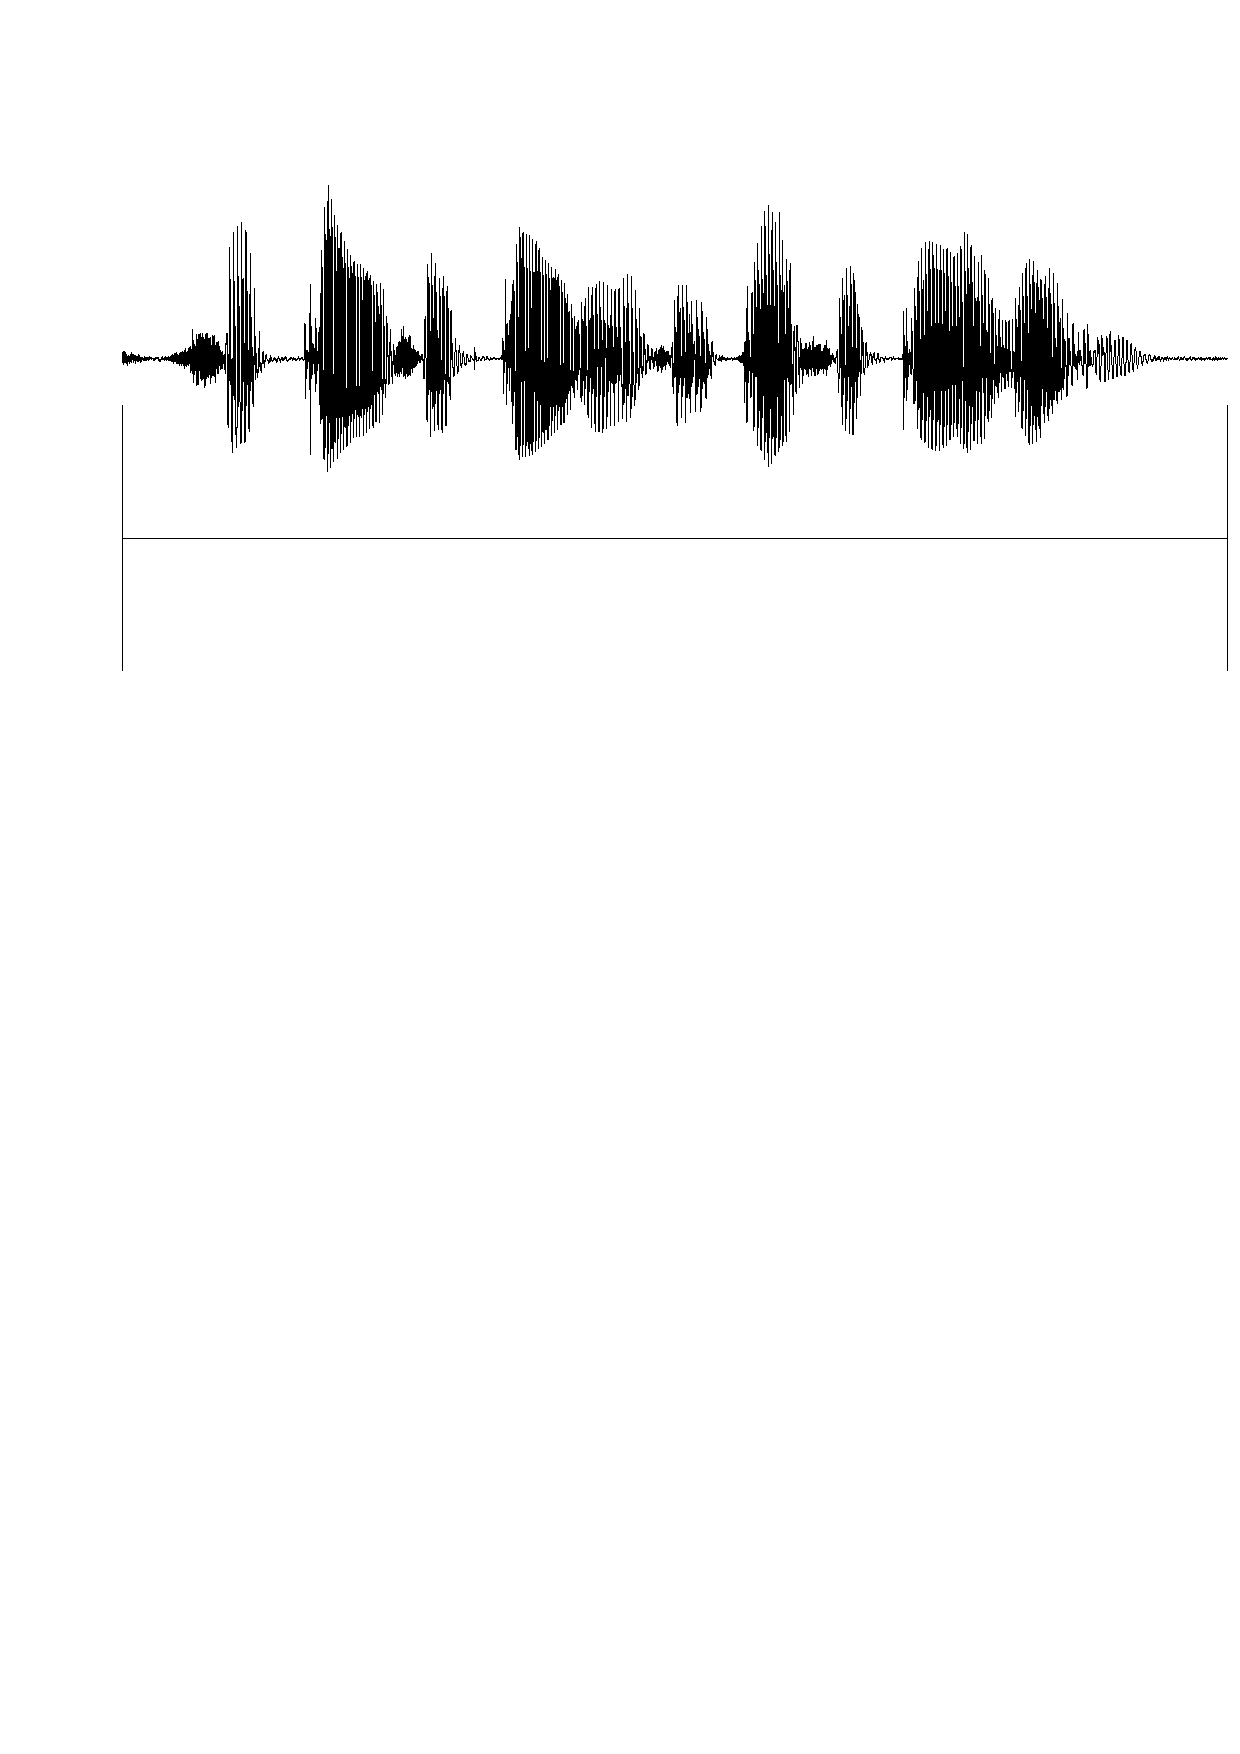
\includegraphics[scale=0.5]{img/default.png}}
      \end{center}
      \end{figure}
    \end{frame}
    
    \begin{frame}{types (stereotypes) vs. tiers}
      \pause
      \begin{figure}[t]
      \setlength{\unitlength}{1cm}
      \begin{center}
      \begin{picture}(12, 8)
          % Symbolic association upper left corner
          \put(1,5.5){Symbolic Association}
          \put(0,7){\line(0,1){0.9}}
          \put(5,7){\line(0,1){0.9}}
          \put(0,7.5){\line(1,0){5}}
          \put(0,6){\line(0,1){0.9}}
          \put(5,6){\line(0,1){0.9}}
          \put(0,6.5){\line(1,0){5}}
        \pause    
          % Symbolic subdivision lower right corner
          \put(7,1.5){Symbolic Subdivision}
          \put(6,2){\line(0,1){0.9}}
          \put(11,2){\line(0,1){0.9}}
          \put(9.5,2){\line(0,1){0.9}}
          \put(7.5,2){\line(0,1){0.9}}
          \put(6,2.5){\line(1,0){5}}
          \put(6,3){\line(0,1){0.9}}
          \put(11,3){\line(0,1){0.9}}
          \put(6,3.5){\line(1,0){5}}
        \pause
          % Included-in lower left corner
          \put(2,1.5){Included In}
          \put(0,3){\line(0,1){0.9}}
          \put(5,3){\line(0,1){0.9}}
          \put(5,3){\line(0,1){0.9}}
          \put(0,3.5){\line(1,0){5}}
          \put(1,2){\line(0,1){0.9}}
          \put(3,2){\line(0,1){0.9}}
          \put(5,2){\line(0,1){0.9}}
          \put(4,2){\line(0,1){0.9}}
          \put(1,2.5){\line(1,0){2}}
          \put(4,2.5){\line(1,0){1}}
       \pause    
          % Time subdivision upper right corner
          \put(7,5.5){Time Subdivision}
          \put(6,6){\line(0,1){0.9}}
          \put(11,6){\line(0,1){0.9}}
          \put(8.5,6){\line(0,1){0.9}}
          \put(10,6){\line(0,1){0.9}}
          \put(7,6){\line(0,1){0.9}}
          \put(6,6.5){\line(1,0){5}}
          \put(6,7){\line(0,1){0.9}}
          \put(11,7){\line(0,1){0.9}}
          \put(6,7.5){\line(1,0){5}}
       \end{picture}
       \end{center}
       \end{figure}
    \end{frame}
    
    \begin{frame}
      \begin{enumerate}
        \item<1-> What \texttt{type} would you create for a \textit{Free Translation} tier?
        \item<2-> What \texttt{type} would you create for a \textit{Word} tier?
        \item<3-> How could you use the \textit{Included In} \texttt{type}?
        \item<4-> Could you use the \textit{Time Subdivision} \texttt{type} for gestures?
      \end{enumerate}
    \end{frame}
    
  % \section{Starting from scratch}
  %   \begin{frame}{starting from scratch}
  %     \begin{enumerate}
  %       \item<1-> Open a sound file (.wav or .mp3)
  %       \item<2-> Save your ELAN file (.eaf)
  %       \item<3-> Create tier types (i.e., \textit{Reference}, \textit{Text}, \textit{Chunk}, \textit{Translation})
  %       \item<4-> Create tiers (i.e., \textit{ref@Speaker} or \textit{HENRY;} or \textit{Intonation Unit})
  %         \begin{itemize}
  %         \item<5-> Select tier types
  %         \item<6-> Set up parent-child relationships
  %         \end{itemize}
  %       \item<7-> Create annotations for your recording
  %     \end{enumerate}
  %   \end{frame}
  %   
  %   \begin{frame}{exercise \# 4 - starting from scratch}
  %     PRACTICE WITH EX \#4 PEAR STORY 
  %     \begin{enumerate}
  %       \item<1-> Open the sound file \texttt{Ex4-ENG-PearStory.mp3}
  %       \item<2-> Save the ELAN file with the same filename
  %       \item<3-> Change the \texttt{default type} to \textit{Text}
  %       \item<4-> Create a \texttt{type} called \textit{Translation} with the stereotype \textit{Symbolic Association}
  %       \item<5-> Start transcribing the text and translate it into your favorite language
  %     \end{enumerate}
  %   \end{frame}
  % 
  %   \begin{frame}{using a template}
  %     \begin{enumerate}
  %       \item<1-> Open sound file (.wav or .mp3) \& template file (.etf or .eaf)
  %       \item<2-> Create annotations for your recording 
  %     \end{enumerate}
  %   \end{frame}
  %   
  %   \begin{frame}{exercise \# 4 - starting with a template}
  %     \begin{enumerate}
  %       \item<1-> Open the sound file \texttt{Ex4-PSE-Andai-andai.wav}
  %       \item<2-> Open the ELAN template \texttt{.etf} file that you created in exercise 3
  %       \item<3-> See the attached text to start creating annotations
  %     \end{enumerate}
  %   \end{frame}
  %   
  % \section{Glossing}
  %   \begin{frame}{glossing words (optional)}
  %     \begin{enumerate}
  %       \item<1-> Open \texttt{Ex5-PSE-20100602-Andai-andai.eaf}.
  %       \item<2-> Tokenize the tier \& create a new tier called \textit{wd@Nining}
  %       \item<3-> Copy the \textit{wd@Nining} \& create a new tier \textit{ge@Nining}
  %       \item<4-> Remove all annotation values (but not the annotations themselves) from the tier
  %       \item<5-> Input the English word translations into the blank annotations
  %     \end{enumerate}
  %   \end{frame}
    
  \section{Conclusion} 
    \begin{frame}{links to further resources}
      \begin{itemize}
        \item ELAN website with manual: \url{http://www.lat-mpi.eu/tools/elan/}
        \item InField course on ELAN: \url{http://logos.uoregon.edu/infield2010/workshops/aligning-text-elan1/index.php}
        \item ELAN tool that incorporates Toolbox functionality: \url{http://corpafroas.tge-adonis.fr/tools.html}
        \item Review of ELAN by Andrea Berez: \url{http://scholarspace.manoa.hawaii.edu/handle/10125/1718/}
      \end{itemize}
    \end{frame}
    
\end{document}